
\begin{resumeBox}
  \emph{À retenir dans une semaine :} 
  \begin{niceitemize}
    \item Nous interprèterons les vecteurs plutôt comme des points, et pas comme des flèches.
    \item Pour résoudre un système linéaire, on le rend \textbf{échelonné} avec le pivot de Gauss.
    \item On peut interpréter un système linéaire de 3 façons différentes : 
      \begin{itemize}
        \item[$\bullet$] Comme une intersection d'éléments géométriques (droites, plans, etc.).
        \item[$\bullet$] Comme une combinaison linéaire de vecteurs.
        \item[$\bullet$] Comme une équation matricielle.
      \end{itemize}
  \end{niceitemize}
\end{resumeBox}
% \begin{formulesBox}
%   % Placez ici vos formules, figures TikZ ou images.
%   % Exemple : $F(\omega)=\int_{-\infty}^{+\infty} f(t)\,e^{-i\omega t}\,dt$
%   % \begin{center}\includegraphics[width=.8\linewidth]{exemple.jpg}\end{center}
% \end{formulesBox}
\begin{rappelsBox}
  \begin{niceitemize}
    \item Que signifie qu'un système soit échelonné ?
    \item Quelles sont les manipulations autorisées pour le pivot de Gauss ?
    \item Comment interpréter un système linéaire comme une combinaison de vecteurs ?
  \end{niceitemize}
\end{rappelsBox}

\section{Exercices}
  \subsection{Équations de réactions chimiques}
  Les équations de réactions chimiques peuvent être interprétées comme des systèmes linéaires. \newline
  Y a-t-il toujours une infinité de façon d'équilibrer l'équation ?


  \vspace{1em}

  Transformer le problème suivant en système linéaire. Sans le résoudre, combien a-t-il de solutions ?
  \begin{center}
    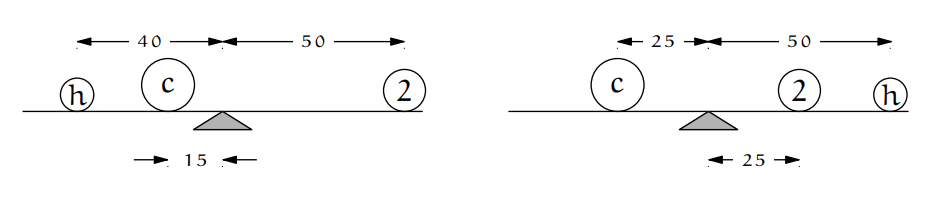
\includegraphics[width=0.8\linewidth]{0-Revisions/2-PivotDeGauss/equilibre.png}
  \end{center}

  \newpage

  \vspace{2em}

  \subsection{Combien de solutions ?}
Ces systèmes admettent-ils zéro, une ou une infinité de solutions ?

% Correction (affichée seulement si showSolutions=true)
\ifthenelse{\boolean{showSolutions}}{}{
  \begin{multicols}{3}
}

\begin{enumerate}[label=\alph*)]
\item $$\begin{cases}
    -3x + 2y &= 0\\
    -2y &= 0
  \end{cases}$$

  \ifthenelse{\boolean{showSolutions}}{
    \vspace{1em}

    \begin{mdframed}
    Le système est bien échelonné avec autant d'équations que d'inconnues, il admet une solution unique.
    \end{mdframed}
}{}


\item $$\begin{cases}
    x + y &= 4\\
    y - z &= 0
  \end{cases}$$

  
\ifthenelse{\boolean{showSolutions}}{
  \vspace{1em}

  \begin{mdframed}
  Le système est déjà échelonné, mais il a plus d'inconnues que d'équations, il admet une infinité de solutions. Ces solutions sont arrangées selon une droite : on peut fixer le paramètre $z$ et exprimer $x$ et $y$ en fonction de $z$.
  \end{mdframed}
}{}

\item 
$$\begin{cases}
    x + y &= 4\\
    y - z &= 0\\
    0 &= 0
  \end{cases}$$

  
\ifthenelse{\boolean{showSolutions}}{
  \vspace{1em}

  \begin{mdframed}
  La dernière équation n'apporte aucune information, c'est le même que le système précédent. 
  \end{mdframed}
}{}
\item 
$$\begin{cases}
    x + y &= 4\\
    0 &= 4
  \end{cases}$$

  
\ifthenelse{\boolean{showSolutions}}{
  \vspace{1em}

  \begin{mdframed}
  La dernière équation est incompatible, le système n'admet pas de solution.
  \end{mdframed}
}{}

\item 
$$\begin{cases}
    3x + 6y + z &= -0.5\\
    -z &= 2.5
  \end{cases}$$

  
\ifthenelse{\boolean{showSolutions}}{
  \vspace{1em}

  \begin{mdframed}
  Le système est échelonné. $2$ équations pour $3$ inconnues, on peut donc en choisir une comme paramètre : $y$,et exprimer $x$ et $z$ en fonction de $y$.
  Il admet donc une droite de solutions.
  \end{mdframed}
}{}


\item 
$$\begin{cases}
    x - 3y &= 2\\
    0 &= 0
  \end{cases}$$

  
\ifthenelse{\boolean{showSolutions}}{
  \vspace{1em}

  \begin{mdframed}
  La dernière équation n'apporte aucune information, On se ramène donc à une équation, deux inconnues. Il y a donc toute une droite de solution.  
  \end{mdframed}
}{}

\item 
$$\begin{cases}
    2x + 2y &= 4\\
    y &= 1\\
    0 &= 4
  \end{cases}$$

  
\ifthenelse{\boolean{showSolutions}}{
  \vspace{1em}

  \begin{mdframed}
  La dernière équation est incompatible, le système n'admet pas de solution.
  \end{mdframed}
}{}
\item 
$$\begin{cases}
    2x + y &= 0
  \end{cases}$$

  
\ifthenelse{\boolean{showSolutions}}{
  \vspace{1em}

  \begin{mdframed}
  C'est l'équation d'une droite. Tous les points de cette droite sont solutions.
  \end{mdframed}
}{}

\item 
$$\begin{cases}
    x - y &= -1\\
    0 &= 0\\
    0 &= 4
  \end{cases}$$

  
\ifthenelse{\boolean{showSolutions}}{
  \vspace{1em}

  \begin{mdframed}
  La dernière équation est incompatible, le système n'admet pas de solution.
  \end{mdframed}
}{}

\item 
$$\begin{cases}
    x + y - 3z &= -1\\
    y - z &= 2\\
    z &= 0\\
    0 &= 0
  \end{cases}$$

  
\ifthenelse{\boolean{showSolutions}}{
  \vspace{1em}

  \begin{mdframed}
  Le système est échelonné, $3$ équations pour $3$ inconnues, il admet une solution unique.
  \end{mdframed}
}{}
\end{enumerate}

\ifthenelse{\boolean{showSolutions}}{}{
\end{multicols}
}


\vspace{2em}
\subsection{Systèmes d'équations linéaires}
Résoudre les systèmes suivants :

% Correction (affichée seulement si showSolutions=true)
\ifthenelse{\boolean{showSolutions}}{}{
\begin{multicols}{3}}
\begin{enumerate}[label={}]
\item 
$$\begin{cases}
  2x + 2y = 5 \\
    x - 4y = 0
  \end{cases}$$

  \ifthenelse{\boolean{showSolutions}}{
        \vspace{1em}

        \begin{mdframed}
        On peut effectuer l'opération $L_2 \leftarrow 2L_2 - L_1$ pour échelonner puis résoudre le système. Il admet une unique solution.
        \end{mdframed}
    }{
    }
\item 
  $$\begin{cases}
    -x + y = 1 \\
    x + y = 2
  \end{cases}$$

  \ifthenelse{\boolean{showSolutions}}{
    \vspace{1em}

    \begin{mdframed}
    On peut effectuer l'opération $L_2 \leftarrow L_2 + L_1$ pour échelonner puis résoudre le système. Il admet une unique solution.
    \end{mdframed}
}{
}

\item 
$$\begin{cases}
    x - 3y + z = 1 \\
    x + y + 2z = 14
  \end{cases}$$

  \ifthenelse{\boolean{showSolutions}}{
    \vspace{1em}

    \begin{mdframed}
    On peut effectuer l'opération $L_2 \leftarrow L_2 - L_1$ pour échelonner puis résoudre le système. Il admet toute une droite de solutions. On pourra choisir $z$ comme paramètre et exprimer $x$ et $y$ en fonction de $z$.
    \end{mdframed}
}{
}

\item 
$$\begin{cases}
    -x - y = 1 \\
    -3x - 3y = 2
  \end{cases}$$

  \ifthenelse{\boolean{showSolutions}}{
        \vspace{1em}

        \begin{mdframed}
        On peut effectuer l'opération $L_2 \leftarrow L_2 + 3L_1$, cela conduit à l'équation $0=5$, qui est incompatible. Le système n'admet pas de solution.
        \end{mdframed}
    }{
    }

\item 
$$\begin{cases}
    4y + z = 20 \\
    2x - 2y + z = 0 \\
    x + z = 5 \\
    x + y - z = 10
  \end{cases}$$

  \ifthenelse{\boolean{showSolutions}}{
    \vspace{1em}

    \begin{mdframed}
      Pour échelonner le système, il faut commencer par échanger les équations pour avoir un $x$ dans la première équation. On échange par exemple $L_1$ et $L_3$. 
      On obtient  
      $$\begin{cases}
          x + z = 5 \\
          4y + z = 20 \\
          2x - 2y + z = 0 \\
          x + y - z = 10
        \end{cases}$$

        Ensuite, on élimine les $x$ des autres équations à l'aide de la première équation : $L_3 \leftarrow L_3 - 2L_1$ et $L_4 \leftarrow L_4 - L_1$. On obtient :
        $$\begin{cases}
          x + z = 5 \\
          4y + z = 20 \\
          -2y - z = -10 \\
           y - 2z = 5
        \end{cases}$$

        Ensuite, on utilise $L_2$ pour éliminer les $y$ : $L_3 \leftarrow 2L_3 + L_2$ et $L_4 \leftarrow 4L_4 - L_2$. On obtient :
        $$\begin{cases}
          x + z = 5 \\
          4y + z = 20 \\
           - z = 0 \\
           - 9z = 0
        \end{cases}$$
        Les 2 dernières équations apportent la même information, on peut en garder seulement une des deux. On obtient un système échelonné avec une unique solution. 
    \end{mdframed}
}{
}


\item 
$$\begin{cases}
    2x + z + w = 5 \\
    y - w = -1 \\
    3x - z - w = 0 \\
    4x + y + 2z + w = 9
  \end{cases}$$

  \ifthenelse{\boolean{showSolutions}}{
    \vspace{1em}

    \begin{mdframed}
      Pour échelonner le système, on peut garder les deux premières équations. On élimine ensuite les $x$ des autres équations à l'aide de la première équation.
      On fait donc : $L_3 \leftarrow 2L_3 - 3L_1$ et $L_4 \leftarrow L_4 - 2L_1$. On obtient :

      $$\begin{cases}
      2x + z + w = 5 \\
      y - w = -1 \\
      -5z - 5w = -15 \\
      y  -w = -1
    \end{cases}$$

    Ensuite, on utilise $L_2$ pour éliminer les $y$ : $L_4 \leftarrow L_4 - L_2$. On obtient :
    $$\begin{cases}
      2x + z + w = 5 \\
      y - w = -1 \\
      -5z - 5w = -15 \\
      0 = 0
    \end{cases}$$

    Le système est échelonné, $3$ équations pour $4$ inconnues, il admet une droite de solutions. On peut choisir $w$ comme paramètre et exprimer $x$, $y$ et $z$ en fonction de $w$.


    \end{mdframed}
}{
}

\end{enumerate}

\ifthenelse{\boolean{showSolutions}}{}{
\end{multicols}}

\vspace{2em}

\subsection{Approfondissement}
Résoudre 
$$\begin{cases}
  2 \sin \alpha-\cos \beta+3 \tan \gamma &= 3 \\
  4 \sin \alpha+2 \cos \beta-2 \tan \gamma &= 10 \\
  6 \sin \alpha-3 \cos \beta+\tan \gamma &= 9
\end{cases}$$

\ifthenelse{\boolean{showSolutions}}{
    \vspace{1em}

    \begin{mdframed}

    On peut se ramener à un système linéaire en posant $x=\sin\alpha$, $y=\cos\beta$, $z=\tan\gamma$. On obtient :
    $$\begin{cases}
      2x - y + 3z = 3 \\
      4x + 2y - 2z = 10 \\
      6x - 3y + z = 9
    \end{cases}$$
    
    On applique alors le pivot de Gauss, on applique $L_2 \leftarrow L_2 - 2L_1$ et $L_3 \leftarrow L_3 - 3L_1$. On obtient :
    $$\begin{cases}
      2x - y + 3z = 3 \\
      0 + 4y - 8z = 4 \\
      0 + 0 - 8z = 0
    \end{cases}$$

    On obtient une unique solution : $x=1/2$, $y=1$, $z=0$.

    On en déduit les solutions de système initial : 
    $$ \alpha = \pi/6 \mod 2\pi \text{ ou } \alpha = 5\pi/6 \mod 2\pi,$$
    $$ \beta = 0 \mod 2\pi,$$
    $$ \gamma = 0 \mod \pi.$$

    \end{mdframed}
}{}


\ifthenelse{\boolean{showSolutions}}{}{
\newpage}
\vspace{2em}

\subsection{Manipulation}

\textit{La méthode de Gauss consiste à combiner les équations d'un système pour en former de nouvelles.}

\medskip
\begin{enumerate}[label=\alph*)]
\item Peut-on obtenir l'équation \(3x - 2y = 5\) par une suite d'opérations de réduction de Gauss à partir des équations de ce système ?
\[
\begin{cases}
x + y = 1 \\
4x - y = 6
\end{cases}
\]

\ifthenelse{\boolean{showSolutions}}{
  \vspace{1em}

  \begin{mdframed}

    Soit on voit tout de suite que $L_2-L_1$ donne $3x-2y=5$.

    Sinon, il faut chercher $a$ et $b$ tels que $aL_1+bL_2$ donne $3x-2y=5$. On obtient le système de $3$ équations à $2$ inconnues :
    $$\begin{cases}
      \text{coefficients devant x : } \quad a + 4b = 3 \\
      \text{coefficients devant y : } \quad a - b = -2 \\
      \text{coefficients du second membre : } a + 6b = 5
    \end{cases}$$

    On obtient donc le système :
    $$\begin{cases}
      a + 4b = 3 \\
      a - b = -2 \\
      a + 6b = 5
    \end{cases}$$
    
    On applique alors le pivot de Gauss, on applique $L_2 \leftarrow L_2 - L_1$ et $L_3 \leftarrow L_3 - L_1$. On obtient :
    $$\begin{cases}
      a + 4b = 3 \\
      0 - 5b = -5 \\
      0 + 2b = 2
    \end{cases}$$
    
    On obtient donc $a=1$ et $b=2$, c'est la seule solution.

  \end{mdframed}
}{
}

\item Peut-on obtenir l'équation \(5x - 3y = 2\) par une suite d'opérations de réduction de Gauss à partir des équations de ce système ?
\[
\begin{cases}
2x + 2y = 5 \\
3x + y = 4
\end{cases}
\]

\ifthenelse{\boolean{showSolutions}}{
  \vspace{1em}

  \begin{mdframed}
    On procède de même, on cherche $a$ et $b$ tels que $aL_1+bL_2$ donne $5x-3y=2$. On obtient le système de $3$ équations à $2$ inconnues :
    $$\begin{cases}
      \text{coefficients devant x : } \quad 2a + 3b = 5 \\
      \text{coefficients devant y : } \quad 2a + b = -3 \\
      \text{coefficients du second membre : } 5a + 4b = 2
    \end{cases}$$

    ce qui conduit au système :
    $$\begin{cases}
      2a + 3b = 5 \\
      2a + b = -3 \\
      5a + 4b = 2
    \end{cases}$$

    On applique alors le pivot de Gauss, on fait $L_2 \leftarrow L_2 - L_1$ et $L_3 \leftarrow 2L_3 - 5L_1$. On obtient :
    $$\begin{cases}
      2a + 3b = 5 \\
      0 - 2b = -8 \\
      0 -7b = -21
    \end{cases}$$
    
    Les deux dernières équations sont incompatibles, le système n'admet pas de solution.
    

  \end{mdframed}
}{
}

\item Peut-on obtenir \(6x - 9y + 5z = -2\) par une suite d'opérations de réduction de Gauss à partir des équations de ce système ?
\[
\begin{cases}
2x + y - z = 4 \\
6x - 3y + z = 5
\end{cases}
\]

\ifthenelse{\boolean{showSolutions}}{
  \vspace{1em}

  \begin{mdframed}
    On procède de même, on cherche $a$ et $b$ tels que $aL_1+bL_2$ donne $6x-9y+5z=-2$. On obtient le système de $3$ équations à $3$ inconnues :
    $$\begin{cases}
      \text{coefficients devant x : } \quad 2a + 6b = 6 \\
      \text{coefficients devant y : } \quad a - 3b = -9 \\
      \text{coefficients devant z : } \quad -a + b = 5 \\
      \text{coefficients du second membre : } 4a + 5b = -2
    \end{cases}$$

  On obtient donc le système :
  $$\begin{cases}
    2a + 6b = 6 \\
    a - 3b = -9 \\
    -a + b = 5 \\
    4a + 5b = -2
  \end{cases}$$

  On applique alors le pivot de Gauss, on fait $L_2 \leftarrow 2L_2 - L_1$ et $L_3 \leftarrow 2L_3 + L_1$ et $L_4 \leftarrow L_4 - 2L_1$. On obtient :
  $$\begin{cases}
    2a + 6b = 6 \\
    -12b = -24 \\
    8b = 16 \\
    -7b = -14
  \end{cases}$$
  Les trois dernières équations sont les mêmes, on obtient un système parfaitement échelonné avec une unique solution : $b=2$ et $a =-3$.

  \end{mdframed}
}{
}


\end{enumerate}


\vspace{2em}
\subsection{Interprétation}
Choisir 3 systèmes linéaire dans un exercice précédent et l'écrire des 2 manières différentes : 
\begin{enumerate}
\item Comme une combinaison linéaires de vecteurs.
\item Comme une équation matricielle.
\end{enumerate}

Par exemple, le système 
$$\begin{cases}
x + y = 1 \\
4x - y = 6
\end{cases}$$
peut s'écrire comme une combinaison linéaire de vecteurs :
$$x\begin{pmatrix}1\\4\end{pmatrix} + y\begin{pmatrix}1\\-1\end{pmatrix} = \begin{pmatrix}1\\6\end{pmatrix}$$
ou comme une équation matricielle :
$$\begin{pmatrix}1&1\\4&-1\end{pmatrix}\begin{pmatrix}x\\y\end{pmatrix} = \begin{pmatrix}1\\6\end{pmatrix}$$



\vspace{2em}
\subsection{Pour ceux qui s'ennuient}
Une boîte contenant des pennies, des nickels et des dimes renferme treize pièces d'une valeur totale de 83 cents.
Combien y a-t-il de pièces de chaque type dans la boîte ?
(Ce sont des pièces américaines : un penny vaut 1 cent, un nickel 5 cents et un dime 10 cents.)


